\chapter{Experimental Setup}
\label{chap:exper_setup}
..intoduce...
\section{The Large Hadron Collider}
\label{sec:LHC}

The Large Hadron Collider (LHC)~\cite{lhcmachine} is a powerful proton-proton synchrotron. It was built and is operated at the European Center for Nuclear Research (CERN) and is situated about 100 m underground close to Geneva, Switzerland. It has a circumference of 26.7 km and uses a tunnel previously built for LEP (Large Electron Positron Collider). Being a particle-particle collider, it consists of two rings with counterrotating beams which are steered using magnets and accelerated using radiofrequency resonating cavities. These beams are made to intersect at four collision points around the LHC ring, at one of which rests the CMS detector. Besides proton-proton collisions the LHC can also collide heavy ions (lead-lead collisions) or heavy ions with protons (lead-proton collisions). Since starting operation in September 2008 the LHC has been the world's most powerful apparatus and will probably remain so in the forseeable future. The following section describes proton-proton collisions at the LHC as the data used in the subsequent physics analysis corresponds to events from these collisions.

The injector chain that supplies protons to the LHC consists of four CERN accelerators that actually predate the LHC: Linac 2, PSB (Proton Synchroton Booster), PS (Proton Synchotron) and SPS (Super Proton Synchotron). This is illustrated in figure~\ref{fig:cern_acc_comp}. The proton source is simply a tank of hydrogen gas. The hydrogen atoms are ionized to yield protons which are then fed in to the Linac 2, a linear accelerator. This accelerates the protons to an energy of about 50 MeV which are then fed into a series of circular accelerators starting with the PSB which accelerates the protons to 1.4 GeV. The PS then accelerates them to 25 GeV, and they are then sent to the SPS which accelerates them to 450 GeV before being finally fed into the LHC beampipe. Inside the LHC the protons are accelerated by sixteen radiofrequency cavities which are made to oscillate at 400 MHz and the proton beam is sorted into discrete packet called 'bunches'. The beam is steered by 1232 Niobium-Titanium superconducting dipole magnets and collimated using quadrupole magnets. This magnet system is kept at a temperature below 2 K, using a pressurised bath of superfluid helium at about 0.13 MPa, and operates at fields above 8T. The LHC has three sophisticated vacuum systems: the insulation vacuum for cryomagnets, the insulation vacuum for  helium  distribution, and the beam vacuum.

\begin{figure*}
\begin{center}
\includegraphics[width=0.8\textwidth,keepaspectratio]{plots_and_figures/chapter3/cern_acc_complex.png}
\caption{Cern Accelerator Complex ~\cite{acc_complex}}
\label{fig:cern_acc_comp}
\end{center}
\end{figure*}


It takes about 4 minutes and 20 seconds to fill up each of the LHC rings wih protons, and about 20 minutes for the proton beam to reach its current peak energy of 6.5 TeV. At this point, each LHC beam contains 2808 bunches with $1.5 \times 10^{11}$ protons per bunch, colliding at a center of mass energy (COM) of 13 TeV. It is anticipated for the COM energy to increase to 14 TeV in 2018. Looking for physics beyond the standard model by colliding protons at such high energies is one of the primary aims of the LHC.

Another important parameter for a collider like the LHC is the instantaneous luminosity (referred to as just luminosity in the following), $\mathscr{L}$. The number of events ($N$) generated per second for some processes is given by:

\begin{equation}
  \frac{dN}{dt}=\sigma\mathscr{L}
\end{equation}


where $\sigma$ is the cross-section of the processes. The luminosity of the LHC can be also expressed in terms of only beam parameters as:

\begin{equation}
  \mathscr{L}=\frac{N_{b}^2 n_{b} f_{rev} \gamma_{r}}{4 \pi \epsilon_{n}\beta^{*}} F
\end{equation}

where $N_{b}$ is number of protons in a bunch, $n_{b}$ is number of bunches per beam, $f_{rev}$ is the revolution frequency, $\gamma_{r}$ the relativistic gamma factor, $\epsilon_{n}$ the transverse beam emittance, $\beta^{*}$ the beta function at the collision point, and F is a reduction factor coming from the fact that the beams cross at an angle.


This luminosity intergrated over time represents the total number of events collected per unit cross section and is called the integrated luminosity ($L$).The LHC has already reached its nominal design luminosity of $10^{34} cm^{-2}s^{-1}$, and it has delivered data amounting to a more than $36 fb^{-1}$, only in 2016. Figure ~\ref{fig:cms_int_lumi} shows the amount of data delivered by the LHC overlaid with the subset collected by the CMS detector in 2015 and 2016.

\begin{figure*}
\begin{center}
  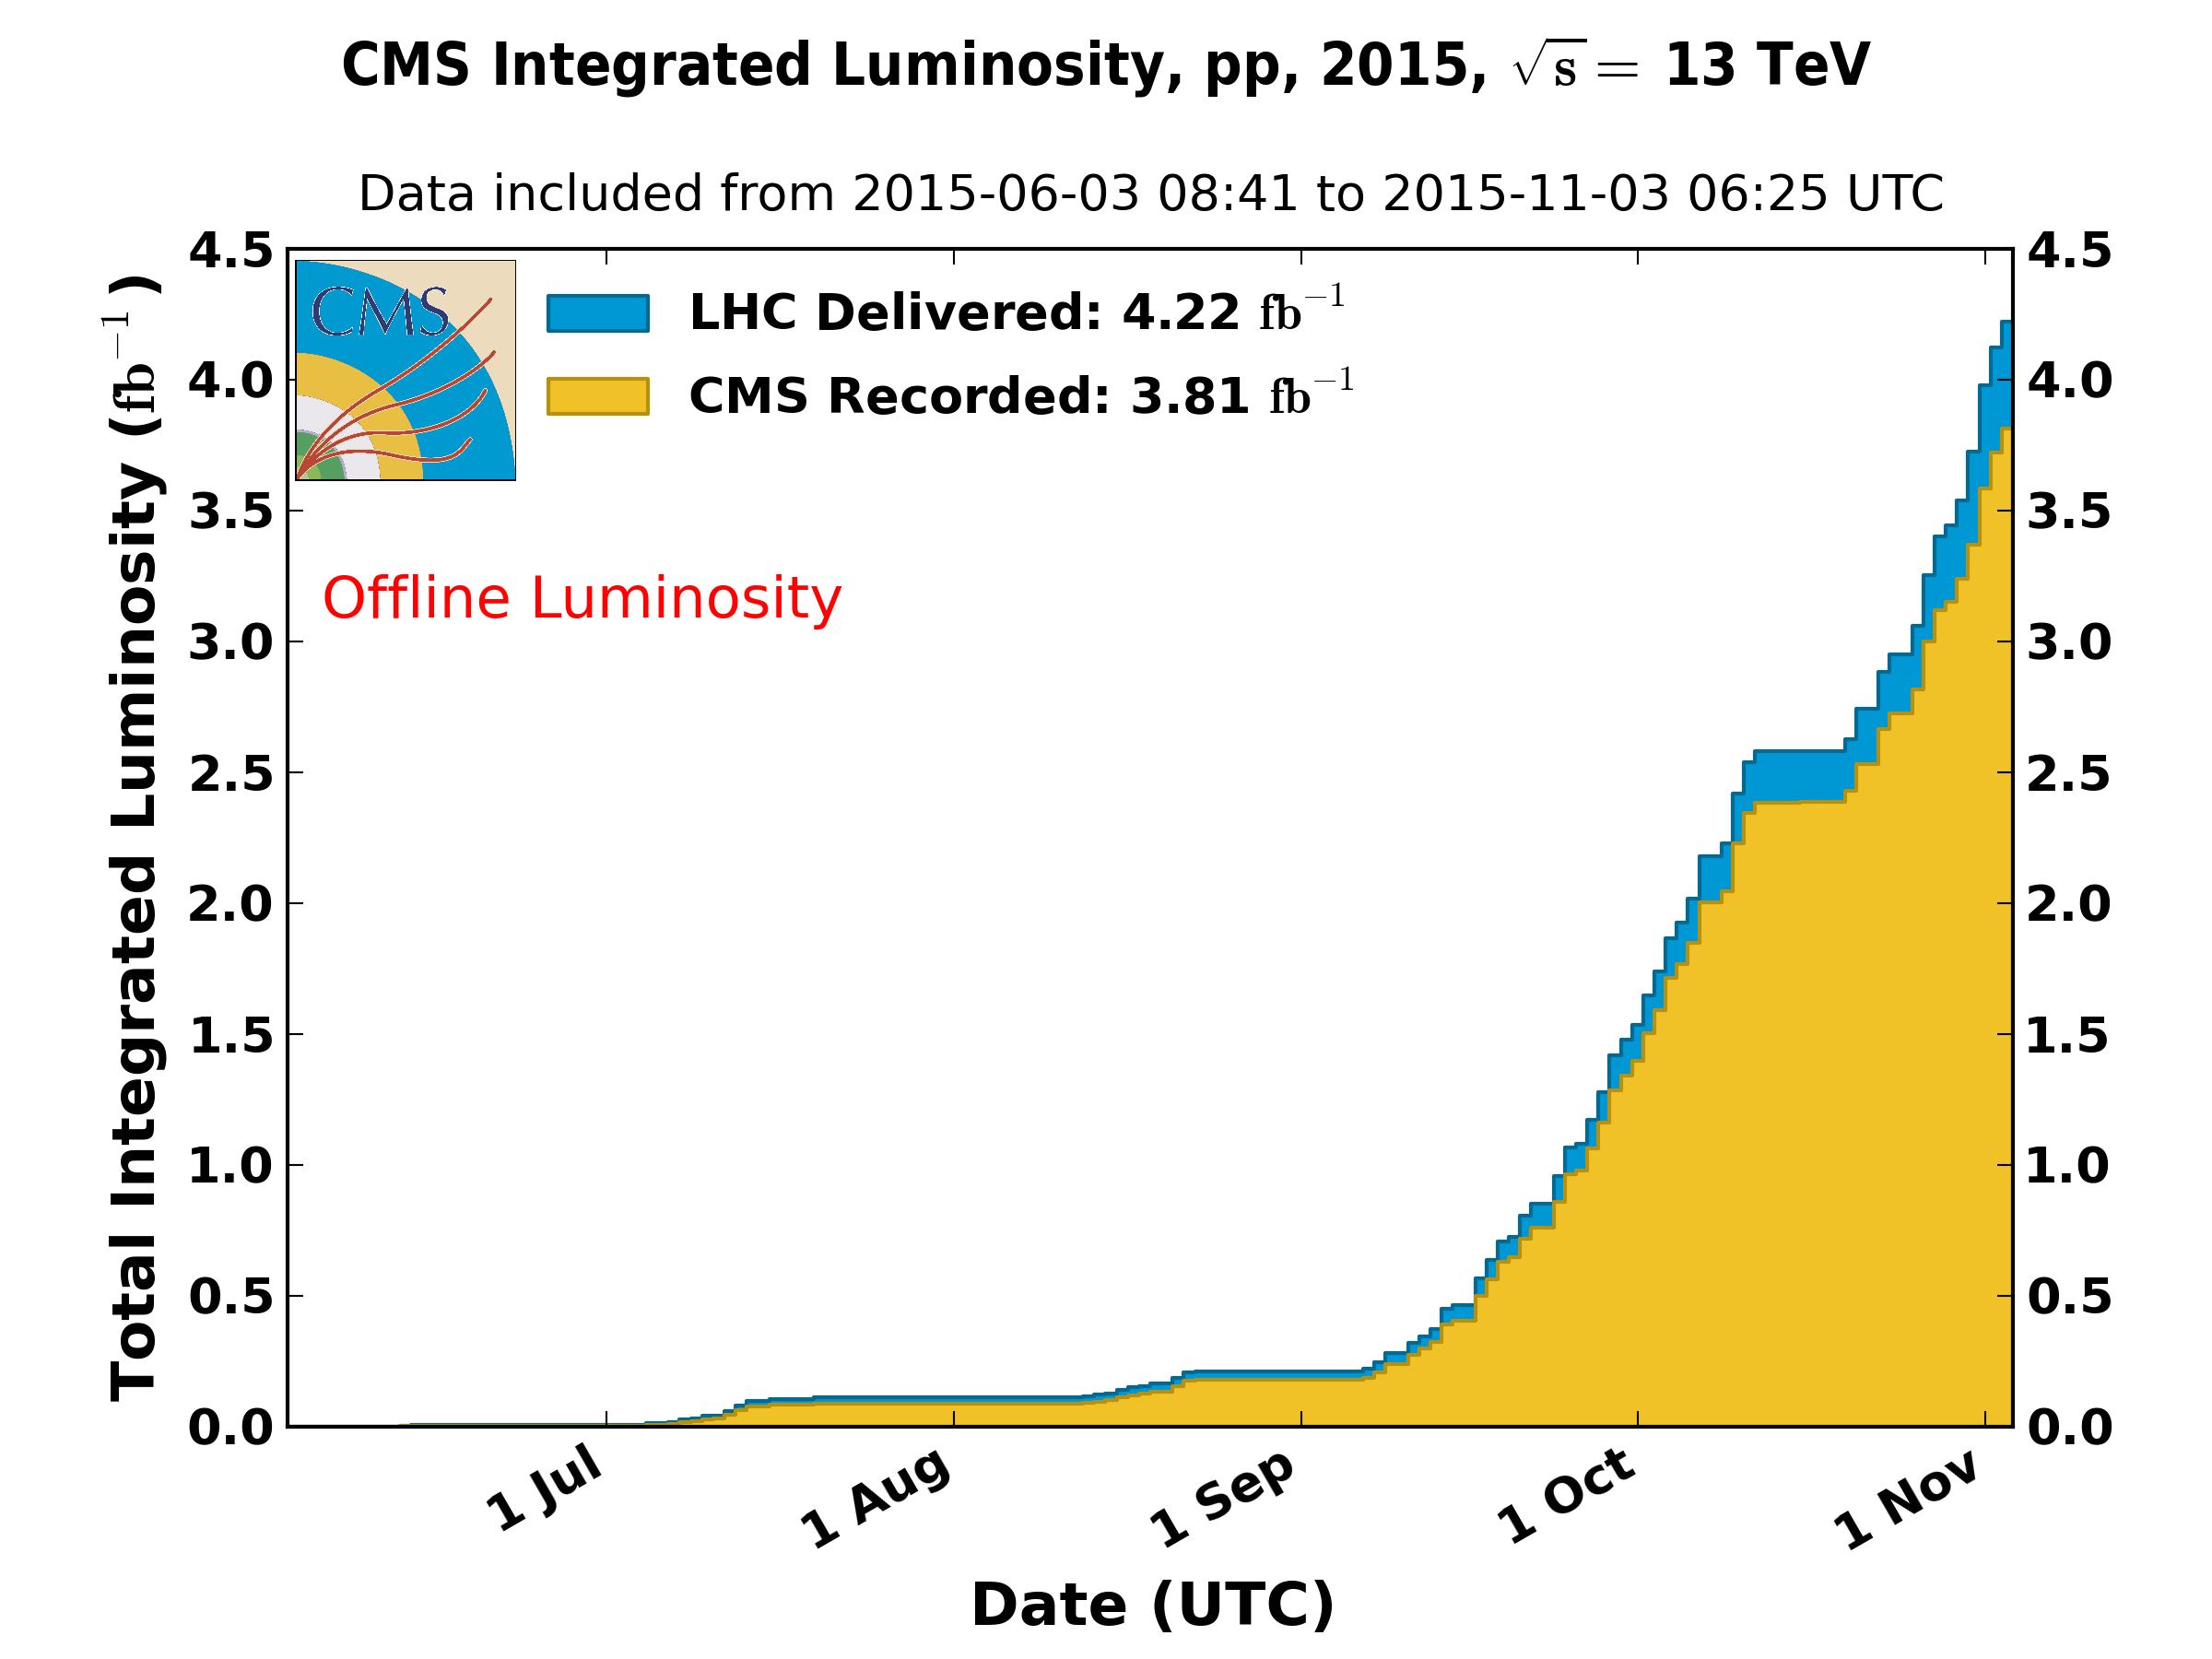
\includegraphics[width=0.4\textwidth,keepaspectratio]{plots_and_figures/chapter3/int_lumi_per_day_cumulative_pp_2015.png}
  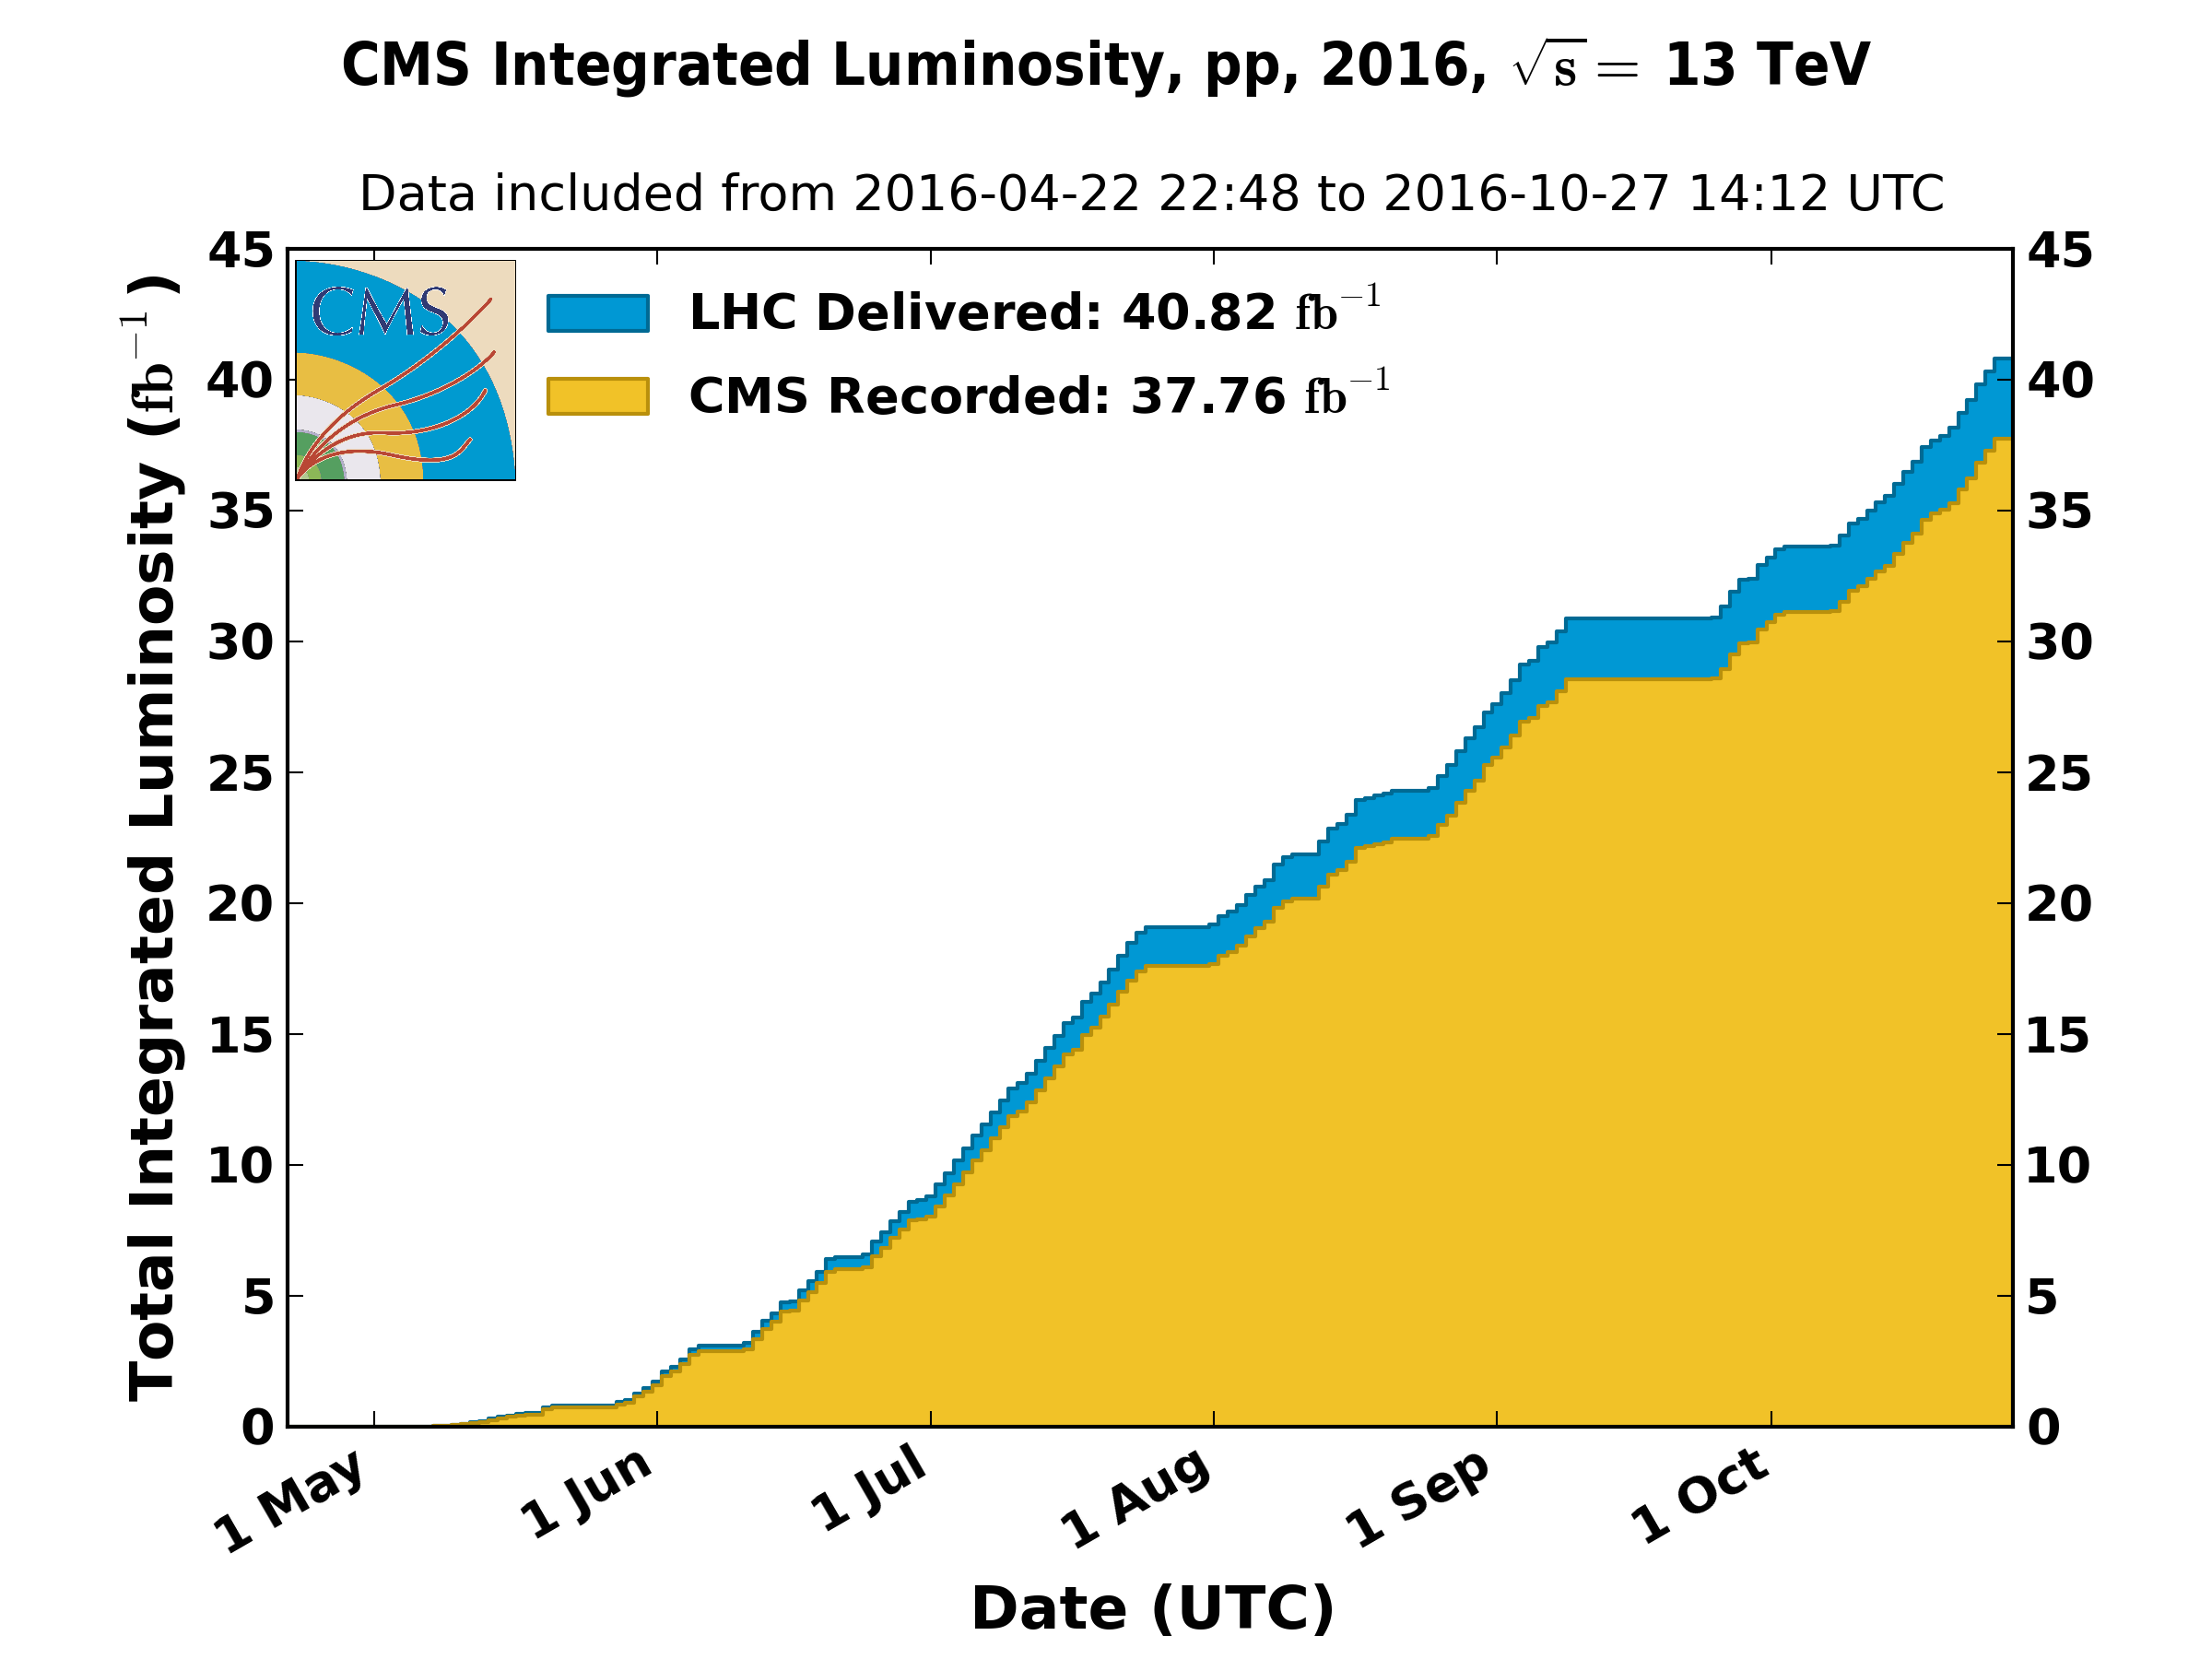
\includegraphics[width=0.4\textwidth,keepaspectratio]{plots_and_figures/chapter3/int_lumi_per_day_cumulative_pp_2016.png}
\caption{Evolution of integrated luminosity in 2015 and 2016 delivered by LHC (blue), and collected by CMS detector (orange)~\cite{cms_int_lumi_ref}.}
\label{fig:cms_int_lumi}
\end{center}
\end{figure*}

In the longer term, it is planned to keep the LHC running, punctuated with several scheduled stops for upgrades and maintenance, at least until late 2030s. During this period it is anticipated to operate at increasingly higher luminosities helping collect unprecedented amounts of data. Figure ~\ref{fig:lhc_schedule} shows an overview of the long term LHC schedule. 
\begin{figure*}
\begin{center}
  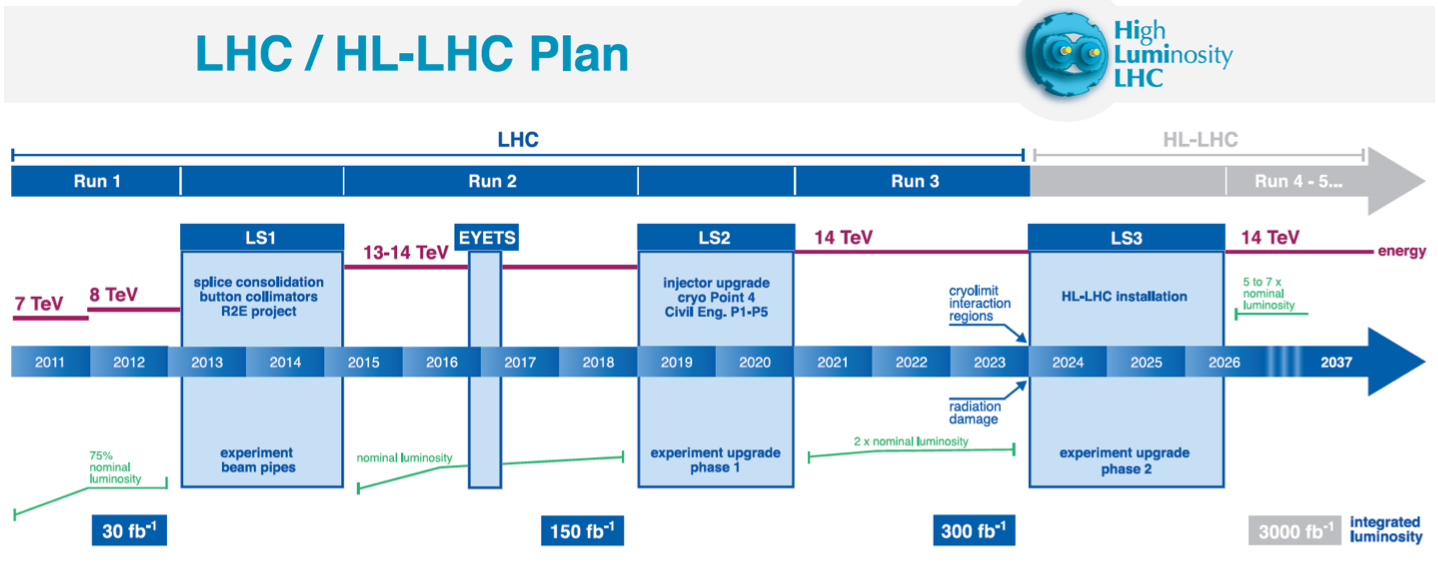
\includegraphics[width=0.95\textwidth,keepaspectratio]{plots_and_figures/chapter3/lhc_schedule.png}
\caption{Overview of the long term LHC schecdule~\cite{LHC_plan_ref}.}
\label{fig:lhc_schedule}
\end{center}
\end{figure*}



\section{The CMS Detector}
\label{sec:CMS}
The Compact Muon Solenoid~\cite{cms_exp_ref} is a general multipurpose particle physics detector that is placed in one of the four collision points of the LHC. It is 28.7m long with a diameter of 15.0m, weighs 14000 tons and is composed of several subdetectors. Its aim is to study a broad array of physics, from making precise measurements of known processess to searches for exotic processes predicted by a multitude of BSM theories. In order to be able to pursue its physics aims at the challenging LHC conditions, the CMS experiment needs to meet several requirements which primarily include good muon identification and momentum resolution over a wide range of momenta and angles, good dimuon mass resolution, good charged-particle momentum resolution and reconstruction efficiency, good electromagnetic energy resolution, good diphoton and dielectron mass resolution, good missing-transverse-energy and dijet-mass resolution.
The backbone of the CMS is a superconducting solenoid that houses its tracking and calorimetry systems and provides an axial magnetic field of 3.8T. The inner-most layer is the silicon pixel and strip tracker that measures the trajectories of charged particles. Surrounding the tracker are the lead tungstate crystal electromagnetic calorimeter (ECAL) which measures the energy of electrons and photons, and the hadronic calorimeter (HCAL) which measures the energy of heavier particles that pass through the ECAL. The ECAL also contains a preshower detector for extra spatial precision. Outside the solenoid is the muon system which has gas-ionization detectors placed in the steel yoke of the magnet. This is the outermost component of CMS and measures the momenta of muons that traverse through it. A sophisticated two-level trigger system that helps filter out a small fraction of most interesting events among millions produced at the LHC also forms a vital part of the CMS.The powerful solenoid, sophisticated muon system and its compact design (given its complexity) give CMS its name. Figure ~\ref{fig:cms_layered} shows a layered view of the detector. The following sections describe it in further detail.   

\begin{figure*}
\begin{center}
  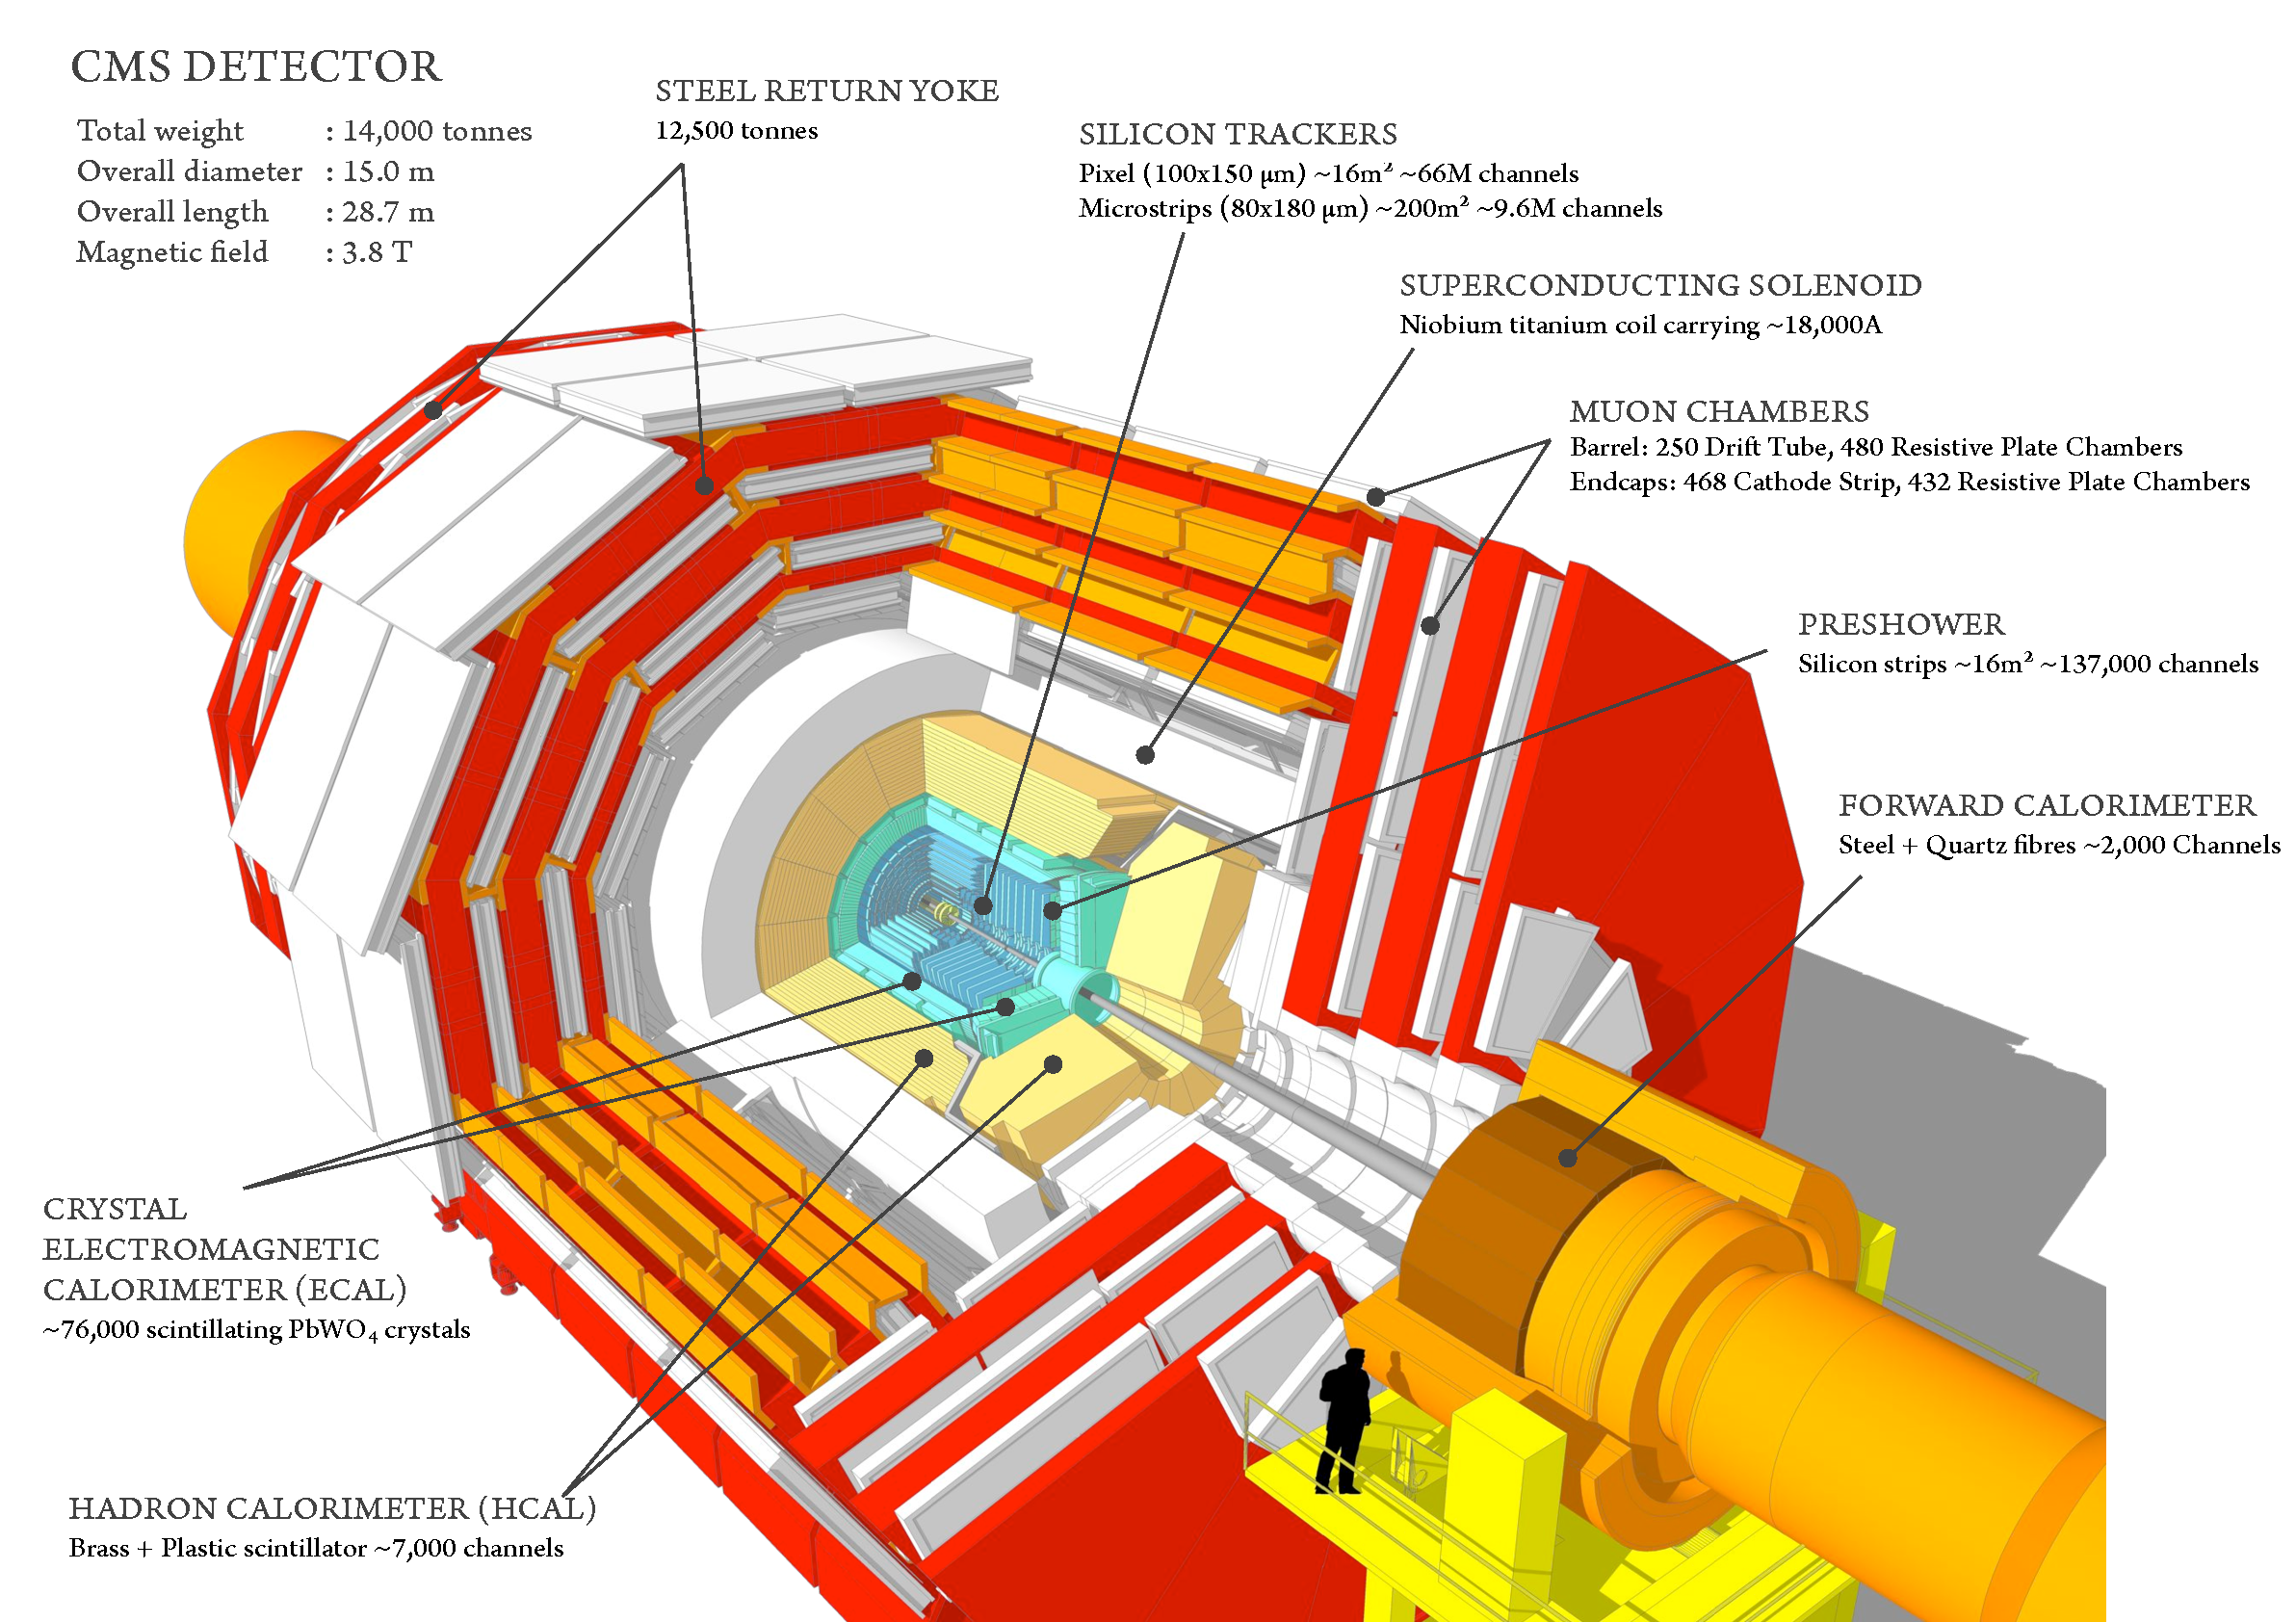
\includegraphics[width=0.95\textwidth,keepaspectratio]{plots_and_figures/chapter3/cms_layered.png}
\caption{Layered View of the CMS detector}
\label{fig:cms_layered}
\end{center}
\end{figure*}




\subsection{Coordinate Conventions}
\label{cor_conv}
The CMS detector has adopted a right-handed coordinate system, the origin of which lies at the nominal collision point inside the experiment.The x-axis points radially inward towards the center of the LHC while the y-axis points vertically upwards. This makes the z-axis point along the beam direction. At point 5 of LHC (a village named Cessy in France) where the CMS is, the z axis points toward the Jura Mountains. In cylindrical co-ordinates, the polar angle $\theta$ is measured from the z-axis while the azimuthal angle $\phi$ is measured from the x-axis in the x-y plane. The polar angle is used to define the pseudo-rapidity $\eta =-ln(tan(\frac{\theta}{2}))$ which is a close approximation for rapidity if $E\gg m$. The rapidity is a Lorentz invariant quantity under boosts in the z-direction. Since it is typical of particles that CMS sees to have $E\gg m$, the Lorentz invariance approximately holds for pseudo-rapidity as well. 

\subsection{CMS Trigger}
\label{trigger}

\subsection{Charged Particle Tracking System}
\label{tracker}

\subsection{Electromagnetic Calorimeter}
\label{Ecal}

\subsubsection{ECAL trigger project}
\label{Ecal_trigger}


\subsubsection{Anomaly detection project for ECAL DQM}
\label{Ecal_DQM}

\subsection{Hadronic Calorimeter}
\label{Hcal}

\subsection{Muon System}
\label{muon_system}

\section{Datasets}
\label{datasets}

The data analysed in this search was gathered by the CMS detector in 2016 during proton-proton collisions at the LHC, corresponding to an integrated luminosity of $35.9 fb^{-1}$. This data corresponds to a center-of-mass energy of 13 TeV and a spacing of 25ns between bunch crossings in the LHC with an average of about 30 collisions per bunch crossing. The subset of samples used among all collected by CMS are the ones having at least one isolated muon having transverse energy over 24 GeV, as triggered by the CMS high level isolated muon trigger (HLT\_IsoMu24 in CMS parlance).
